\subsection{Transitions between environment} 
Figure \ref{fig:trans} depicts the typical transition between environments in different homogenous runs. To compute this typical transition we averaged k calculated at iterations $[t-40; t + 40]$ for every $t \in T_r$ of a run $r$ where $T_r$ is the set of every iteration of $r$ when a transitions between environments occurs. Figure  \ref{fig:transonly} shows the different typical transitions of \emph{Short-Cycle Fluctuation} genotypes tested a homogeneous test with the same fluctuations. We can see that phenotypes of the genotypes collected later in the evolutionary process are less sensitive to environmental fluctuations. Conversely, as reported of Figure \ref{fig:transli}, the phenotypes of genotypes from \emph{Short-Cycle Fluctuation} keep the same high sensitivity regardless of the iteration in which they were collected.


\begin{figure}[H]
\begin{subfigure}{.25\textwidth}
  \centering
  \includegraphics[width=.7\linewidth, angle =-90]{img/Failavg499999variationb.eps}
  \caption{Strong Fluctuation.}
  \label{fig:transst}
\end{subfigure}%
\begin{subfigure}{.25\textwidth}
  \centering
  \includegraphics[width=.7\linewidth, angle =-90]{img/avgvarValidvariationb.eps}
  \caption{Strong Fluctuation.}
  \label{fig:transli}
\end{subfigure}

\begin{subfigure}{.25\textwidth}
  \centering
  \includegraphics[width=.7\linewidth, angle =-90]{img/Failavg499999variationSmallb.eps}
  \caption{Short-Cycle Fluctuation.}
  \label{fig:transstest}
\end{subfigure}%
\begin{subfigure}{.25\textwidth}
  \centering
  \includegraphics[width=.7\linewidth, angle =-90]{img/FailavgvarSmallValidvariationSmallb.eps}
  \caption{Short-Cycle Fluctuation.}
  \label{fig:transonly}
\end{subfigure}
\caption{Typical transition between environment in different types of homogenous test.}
\label{fig:trans}
\end{figure}


\subsection{Phenotypic Diversity} 

The phenotypic diversity measured in Figure \ref{fig:phenodiv} can also be observed relatively easily by simple observation of the cellular automaton as it can be seen with a few examples in Figures \ref{fig:phenoexpl}. 



\begin{figure}[H]
\begin{subfigure}{.25\textwidth}
  \centering
  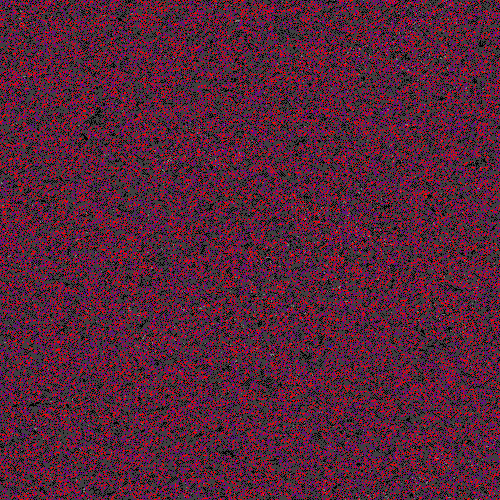
\includegraphics[width=.9\linewidth]{img/stable495000}
  \caption{Stable environment.}
\end{subfigure}%
\begin{subfigure}{.25\textwidth}
  \centering
  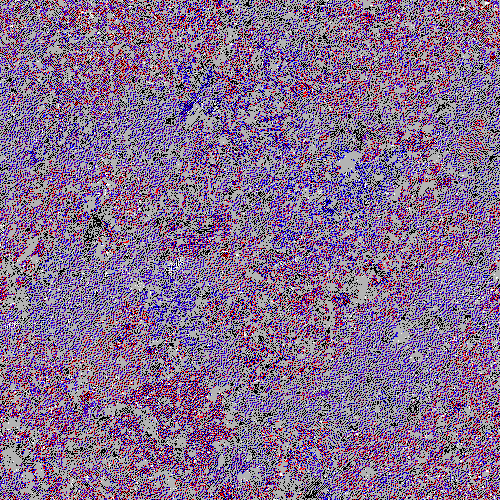
\includegraphics[width=.9\linewidth]{img/var495000}
  \caption{Strong Fluctuation.}
\end{subfigure}

\begin{subfigure}{.25\textwidth}
  \centering
  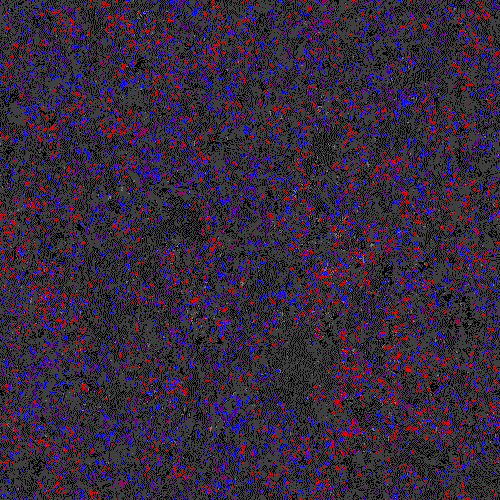
\includegraphics[width=.9\linewidth]{img/light495000}
  \caption{Light Fluctuation.}
\end{subfigure}%
\begin{subfigure}{.25\textwidth}
  \centering
  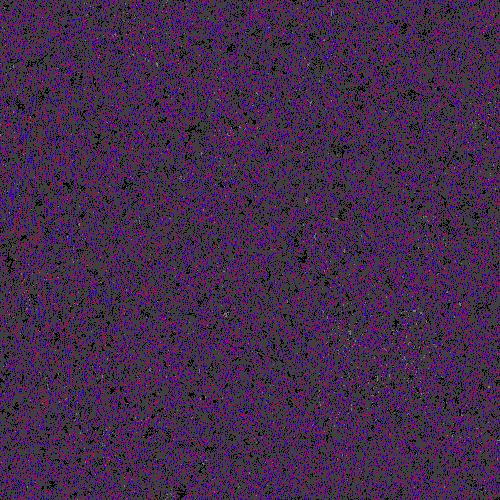
\includegraphics[width=.9\linewidth]{img/small495000}
  \caption{Short-Cycle Fluctuation.}
\end{subfigure}
\caption{Example of CA gird state repartition (phenotype) at iteration 495000 for the four different configuration. Each cell state is represented by a different color. Black and grey represent respectively cells in \emph{decay} and \emph{quiescent} state.}
\label{fig:phenoexpl}
\end{figure}


One distinguishes \emph{Strong and Light fluctuations} from \emph{Short-Cycle fluctuations}. These two groups diverge substantially in their characteristic and differ in addition from \emph{Stable Environment}, frequently in between. Individuals from \emph{Short-Cycle fluctuations} seem to produce stable and robust phenotypes in any environment encountered in \emph{Short-Cycle fluctuations}. Their adaptations seem essentially be by genotypic mutations and their plasticity seems low. They are also very dependent on their original ecosystem, sometime very distinctive as depicted in Figure \ref{fig:smalldistinctive}, and consequently very little robust in other types of fluctuations, the effect of genotypic mutations is probably enhanced by the reduced size of genotypes. By contrast individuals evolved with \emph{Strong or Light fluctuations} appear to have a considerable plasticity, their phenotypic diversity is high and it seems likely that phenotypic selection occurs however their genotypic diversity is lower.

\begin{figure}[H]
\begin{subfigure}{.25\textwidth}
  \centering
  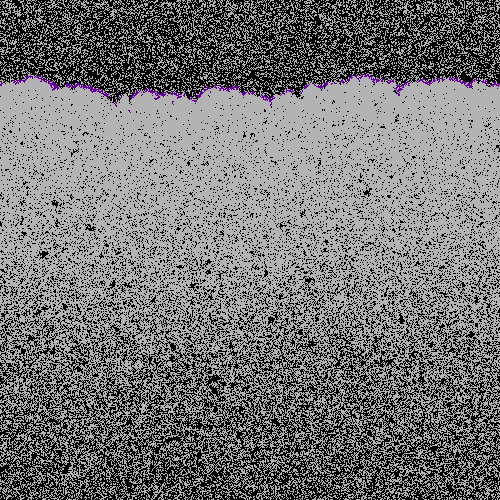
\includegraphics[width=.9\linewidth]{img/sm100000}
  \caption{Iteration 100000.}
\end{subfigure}%
\begin{subfigure}{.25\textwidth}
  \centering
  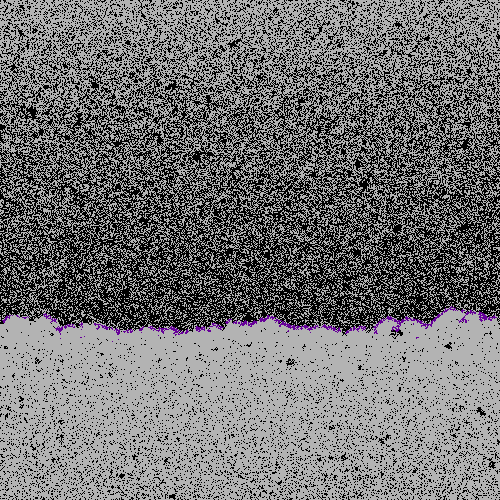
\includegraphics[width=.9\linewidth]{img/sm200000}
  \caption{Iteration 200000.}
\end{subfigure}

\begin{subfigure}{.25\textwidth}
  \centering
  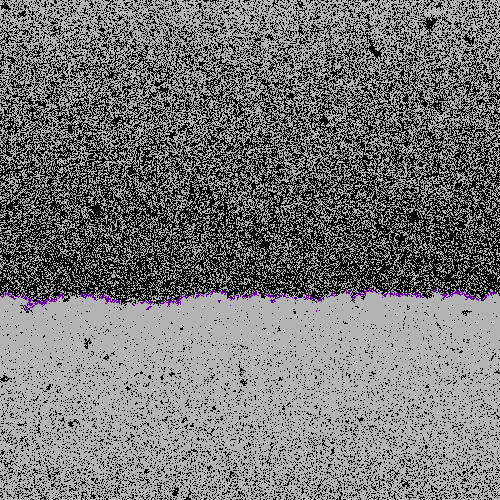
\includegraphics[width=.9\linewidth]{img/sm400000}
  \caption{Iteration 400000.}
\end{subfigure}%
\begin{subfigure}{.25\textwidth}
  \centering
  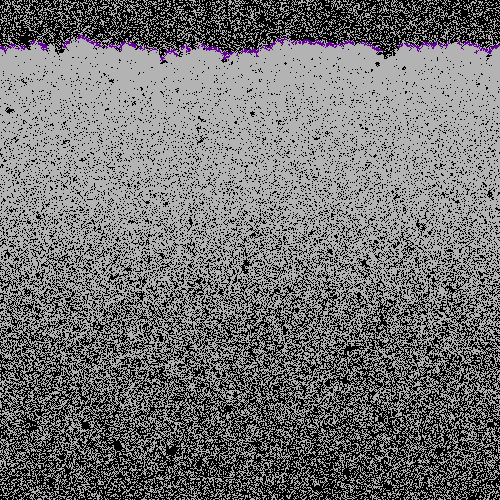
\includegraphics[width=.9\linewidth]{img/sm500000}
  \caption{Iteration 500000.}
\end{subfigure}
\caption{Original \emph{Short-Cycle Fluctuation} simulation having a distinctive waving phenotype, very stable over time, and producing genotypes failing in early iteration of homogeneous test.}
\label{fig:smalldistinctive}
\end{figure}
